\chapter{More on LMMs plus adaptive step-size selection}

This lecture discusses the general form of LMMs and gives a brief 
discussion of step size adaptation and selection for ODE solvers. 

\section{General form of LMMs}

In general a $k$-step LMM method takes the form 
\begin{equation*}
    \sum_{j=0}^k \alpha_j u_{n+j} = \Delta t \sum_{j=0}^k \beta_j f_{n+j},
\end{equation*} 
with coefficients $\alpha_j, \beta_j$ to be identified. 
Replacing $u_{n+j} \leftarrow v(t_{n+j}) = v(t_n + j \Delta t)$ and $f_{n+j} \leftarrow
v'(t_{n+j}) = v'(t_{n} + j \Delta t)$, for a smooth function $v$,
 the LMM is analogous to the identitiy 
\begin{equation}\label{eq:l13-disp1}
    \sum_{j=0}^k \alpha_j v(t_{n} + j \Delta t) 
    = \Delta t \sum_{j=0}^k \beta_j v'(t_{n} + j \Delta t) + \mathcal{O}(\Delta t^{p+1}).
\end{equation}
Then the index $p$ will precisely turn out to be the order of 
consistency of the LMM. Then an LMM can be designed by choosing the 
coefficients $\alpha_j, \beta_j$ to obtain a desired valued of $p$ 
or to just obtain the highest possible value. It turns out many choices 
are possible and give rise to different families of methods. 

A systematic approach for choosing such coefficients is to consider 
the Taylor expansions 
\begin{equation*}
    \begin{aligned}
        v(t_n + j \Delta t) & = \sum_{m=0}^p \frac{v^{(m)}(t_n)}{m!} 
    (j \Delta t)^m + \frac{v^{(p+1)}(\xi_j)}{(p+1)!} 
    (j \Delta t)^{p+1} \\
       \Delta t \cdot v'(t_n + j \Delta t) 
       &= \sum_{m=0}^{p-1} 
       \frac{v^{(m+1)}(t_n)}{m!} 
    j^m (\Delta t)^{m+1} + \frac{v^{(p+1)}(\zeta_j)}{p!} 
    j^{p} (\Delta t)^{p+1} 
    \end{aligned}
\end{equation*}
and substitute them into \eqref{eq:l13-disp1} and 
cancel all terms of  $\mathcal{O}(\Delta t^p)$ and below. 
This gives a system of equations for the model parameters.  
In particular, define
\begin{equation*}
    C_0 = \sum_{j=0}^k \alpha_j 
    \qquad 
    C_m = \sum_{j=0}^k \left( \frac{j^m}{m!} \alpha_j
    - \frac{j^{m-1}}{(m-1)!} \beta_j \right),
    \quad m = 1, \dots, p,
\end{equation*}
where $C_m$ is the coefficient of $v^{(m)}(t_n) \Delta t^m$ in the
difference between the left and right hand sides of
\eqref{eq:l13-disp1}. Then the 
LMM has order $p$ if $C_0 = C_1 = \dots = C_p = 0$. This gives us 
$p+1$ equations. At the same time, the LMM has $2k + 1$ unknown coefficients, 
since we take $\alpha_k = 1$ for simplicity. Thus in principle 
we can have a method of order $p=2k$ without considering other 
issues such as stability. Thus, in practice we can work with $p < 2k$ 
which leaves extra free parameters for us to choose to either 
improve the computational cost of the method or to improve its stability 
properties; see \cite{griffiths2010numerical} for a detailed explanation of 
the stability theory of LMMs.

The above line of thinking gives rise to the many families of LMMs. 
For example, the explicit Adams family takes the general form 
\begin{equation*}
    u_{n+k} - u_{n+k - 1} = \Delta t\sum_{j=0}^{k-1} \beta_j f_{n + j},
\end{equation*}
which is an LMM method where $\alpha_k =1, \alpha_{k-1} = -1$ and 
the rest of the $\alpha_j$'s as well as $\beta_k$ are set to zero. 
The choice of $\beta_k = 0$ is crucial because it makes sure 
the method is explicit. 

Alternatively, the implicit Adams family takes the form 
\begin{equation*}
    u_{n+k} - u_{n+k - 1} = \Delta t\sum_{j=0}^{k} \beta_j f_{n + j},
\end{equation*}
notice that the only difference is that we now included 
$\beta_k$ in the sum which makes the method implicit. Finally, 
the so-called Bakcwards Differentiation Formula (BDF) family takes 
the general form 
\begin{equation*}
    \sum_{j=0}^k \alpha_j u_{n+j} = \Delta t \beta_k f_{n+k}.
\end{equation*} 
This family is popular for solving stiff problems and can be viewed as a 
generalization of backward Euler.

\section{Adaptive step-size selection}

So far in the course we have primarily considered algorithms with 
fixed step sizes, i.e., we assumed $t_{n} - t_{n-1} = \Delta t$ 
which is fixed. In practice, such a fixed choice is often sub-optimal 
since varying the step-size can allow us to obtain more 
efficient algorithms. 

As an example, consider the stiff ODE \eqref{eq:stiff-ODE-example}
and suppose we want to solve it using forward Euler. Since the problem 
is stiff we need to choose a very small $\Delta t$ at the beginning 
but later the solution is nice and smooth and we can choose a much 
larger value of $\Delta t$; see \Cref{fig:adaptive-forward-Euler}.
The trick to making such a method work is to allow for 
the update rules to use different step sizes, i.e., we use 
\begin{equation*}
    u_{n+1} = u_n + \Delta t_n f_n,
\end{equation*}
which is simple enough. However, the important question is 
how should we choose $\Delta t_n$? A simple approach for 
this is to try to estimate the truncation error of the 
method. In particular, for forward Euler, we recall that 
\begin{equation*}
    u(t_{n+1}) - u(t_n) + \Delta t_n f(t_n, u(t_n)) 
    = \frac{ \Delta t_n^2}{2} u''(\xi),
\end{equation*}
where $\xi \in [t_n, t_{n+1}]$.
On the other hand 
\begin{equation*}
    u''(\xi) \approx \frac{1}{\Delta t} 
    \Big( u'(t_{n+1}) - u'(t_n) \Big)
    = \frac{1}{\Delta t} \Big(
    f(t_{n+1}, u(t_{n+1})) - f(t_{n}, u(t_{n})) \Big). 
\end{equation*}
Thus, for the numerical solution, we can simply choose $\Delta t_n$ 
such that 
\begin{equation}\label{eq:l13-disp2}
    \frac{ \Delta t_n^2 }{2} | f_{n+1} - f_n| \le \text{TOL}.
\end{equation}
This is efficient because if our proposed $\Delta t_n$ is accepted 
then we can directly use $f_{n+1}$ to compute our forward Euler step 
at no cost. 


Various strategies exist for adaptation of the 
$\Delta t_n$ that are beyond the scope of the course. A simple 
approach is to start with the error estimate 
\begin{equation*}
    \text{ERROR} =  \frac{ [\Delta t_n]_{\text{old}}^2 }{2} | f_{n+1} - f_n| 
    \approx C [\Delta t_n]_{\text{old}}^2,
\end{equation*}
where we wrote $[\Delta t_n]_{\text{old}}$ to denote the step-size 
that needs to be updated.
Then we can estimate $C = \frac{\text{ERROR}}{[\Delta t_n]_{\text{old}}^2}$. 
At the same time, we want $C [\Delta t_n]_{\text{new}}^2 = \text{TOL}$, 
where we now write $[\Delta t_n]_{\text{new}}$ to denote the 
updated step-size to be chosen. 
Thus, using the estimate for $C$ we obtain a recursive formula 
to update $\Delta t_n$ at each step 
\begin{equation*}
    [\Delta t_n]_{\text{new}} \leftarrow \left( \frac{TOL}{C} \right)^{1/2}
    = [\Delta t_n]_{\text{old}} \left( \frac{TOL}{ERROR} \right)^{1/2}. 
\end{equation*}
We iterate this formula until our $\Delta t_n$ choice 
passes \eqref{eq:l13-disp2}. Note that the above 
formula has the benefit that it allows $\Delta t_n$ to 
naturally decrease but also increase should our error be 
much smaller than the tolerance.  In practice we often supplement 
this update with an extra safety parameter 
\begin{equation*}
    [\Delta t_n]_{\text{new}} \leftarrow  s \cdot [\Delta t_n]_{\text{old}} \left( \frac{TOL}{ERROR} \right)^{1/2}. 
\end{equation*}
where $s \in (0, 1]$ is a tuning parameter. 


\begin{figure}
    \centering
    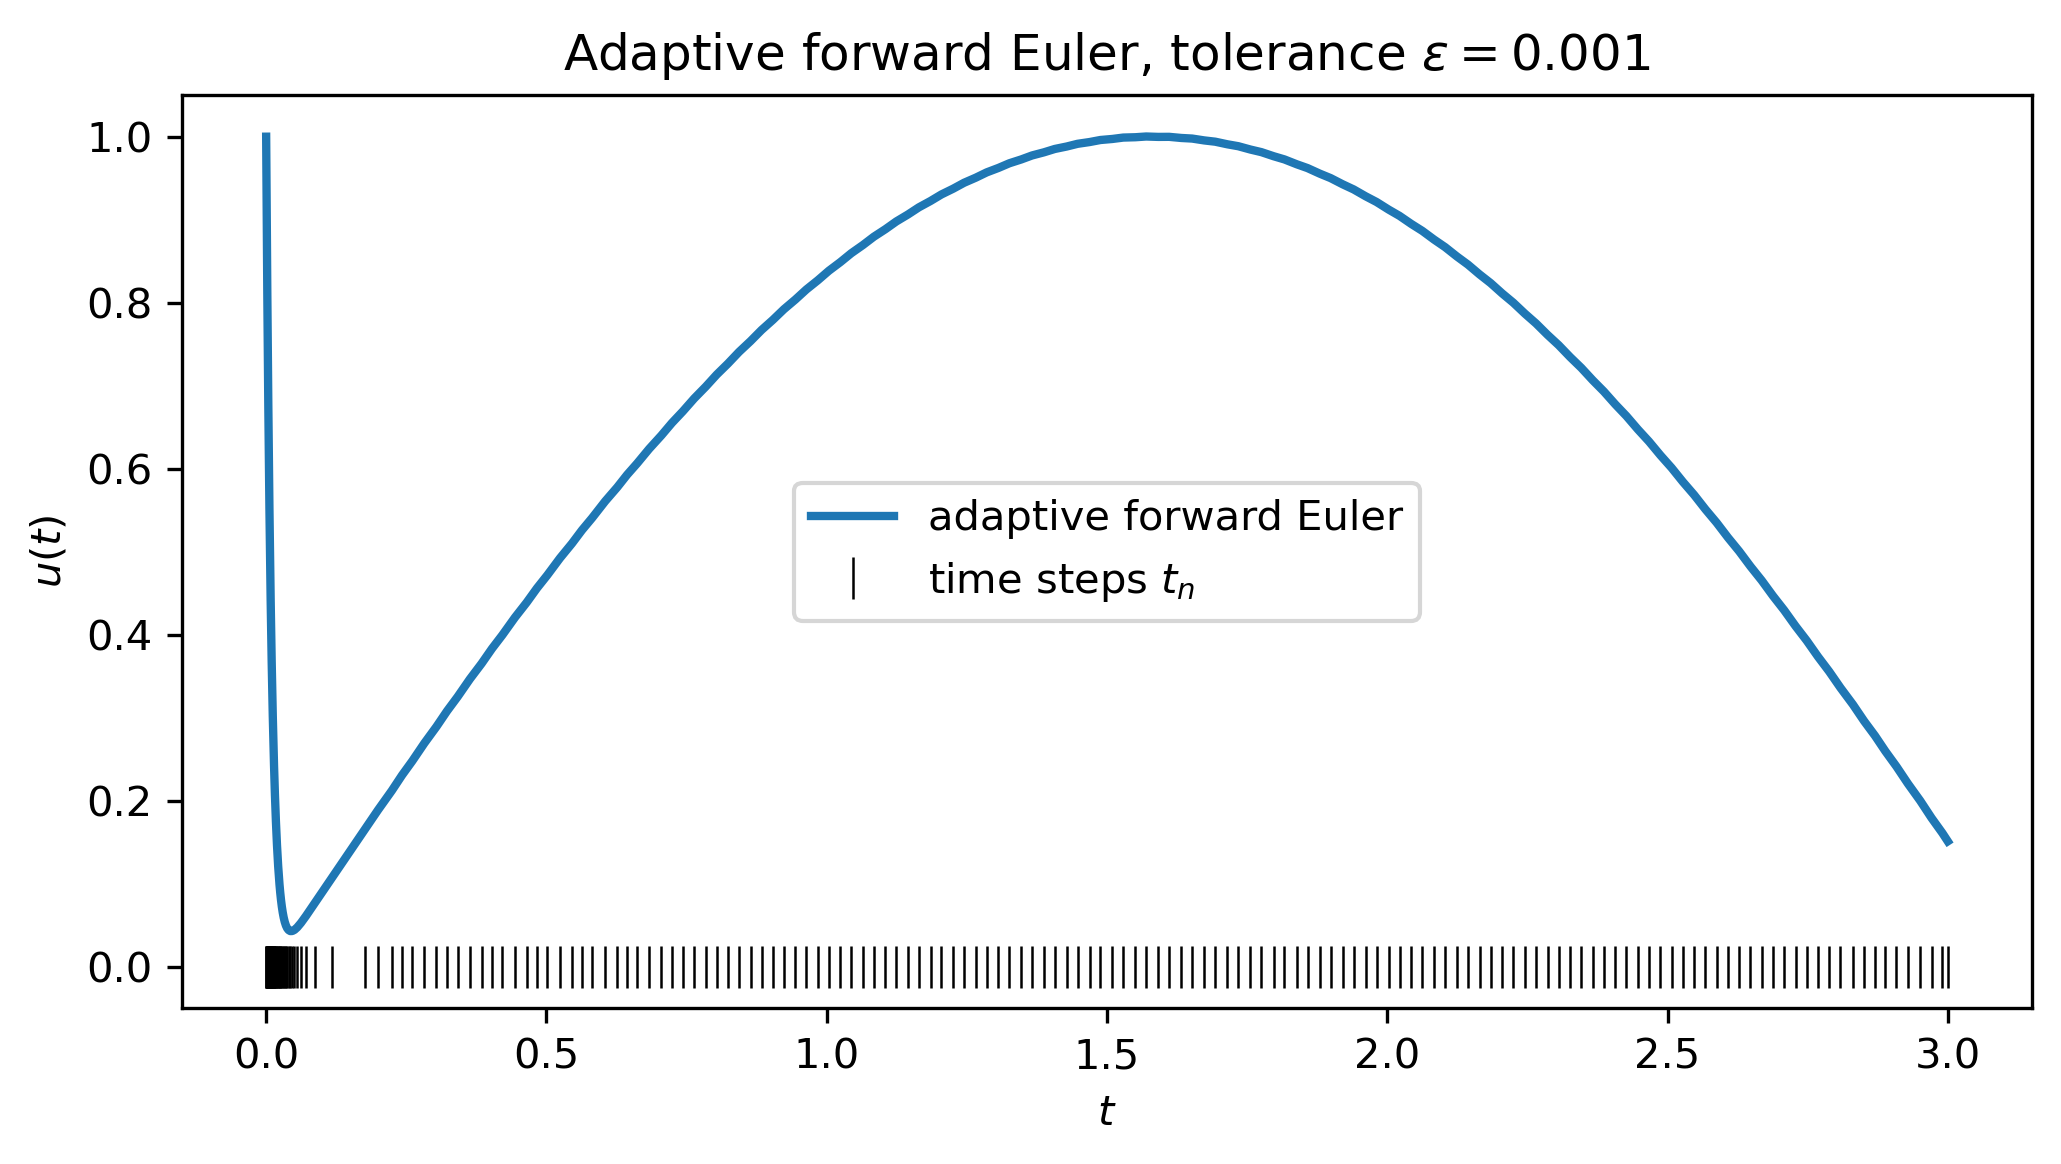
\includegraphics[width=0.6 \textwidth]{./Lectures/Lec13/adaptive_forward_euler.png}
    \caption{An instance of forward Euler with adaptive step sizes 
    chosen to control the local truncation errors below tolerance 
    $10^{-3}$.}
    \label{fig:adaptive-forward-Euler}
\end{figure}





\bibliographystyle{plainnat}
\bibliography{references}